% LaTeX template for DLD Lab - runs with MikTeX and other platforms

\documentclass{article}
\usepackage{mathptmx}
\usepackage{amssymb}
\usepackage{amsfonts}
\usepackage{amsmath}
\usepackage{latexsym}
\usepackage{setspace}
\usepackage{verbatim}

\usepackage[dvipsnames]{xcolor}
\usepackage{matlab-prettifier}
\usepackage{float}
\usepackage[export]{adjustbox}



\numberwithin{equation}{section}
\newtheorem{thm}{Theorem}[section]
\newtheorem{dfn}[thm]{Definition}
\newtheorem{lem}[thm]{Lemma}
\newtheorem{rem}[thm]{Remark}
\newtheorem{cor}[thm]{Corollary}
\newtheorem{prop}[thm]{Proposition}
\newtheorem{asm}[thm]{Assumption}
\newtheorem{example}[thm]{Example}

\newenvironment{proof}{\noindent {\bf Proof.\/}}{$\qed$\vskip 0.1in}
\def\qed{ \hfill \vrule width.2cm height.2cm depth0cm\smallskip}

\usepackage{xcolor}
\usepackage{listings}
\usepackage{pythonhighlight}

\definecolor{mGreen}{rgb}{0,0.6,0}
\definecolor{mGray}{rgb}{0.5,0.5,0.5}
\definecolor{mPurple}{rgb}{0.58,0,0.82}
\definecolor{backgroundColour}{rgb}{0.95,0.95,0.92}

\lstdefinestyle{CStyle}{
    backgroundcolor=\color{backgroundColour},   
    commentstyle=\color{mGreen},
    keywordstyle=\color{magenta},
    numberstyle=\tiny\color{mGray},
    stringstyle=\color{mPurple},
    basicstyle=\footnotesize,
    breakatwhitespace=false,         
    breaklines=true,                 
    captionpos=b,                    
    keepspaces=true,                 
    numbers=left,                    
    numbersep=5pt,                  
    showspaces=false,                
    showstringspaces=false,
    showtabs=false,                  
    tabsize=2,
    language=C
}

\DeclareMathOperator*{\argmax}{argmax} % thin space, limits underneath in displays


% For minted -> Python
\usepackage{tcolorbox}
\tcbuselibrary{minted,breakable,xparse,skins}
\definecolor{bg}{gray}{0.95}
\DeclareTCBListing{mintedbox}{O{}m!O{}}{%
  breakable=true,
  listing engine=minted,
  listing only,
  minted language=#2,
  minted style=default,
  minted options={%
    linenos,
    gobble=0,
    breaklines=true,
    breakafter=,,
    fontsize=\small,
    numbersep=8pt,
    #1},
  boxsep=0pt,
  left skip=0pt,
  right skip=0pt,
  left=25pt,
  right=0pt,
  top=3pt,
  bottom=3pt,
  arc=5pt,
  leftrule=0pt,
  rightrule=0pt,
  bottomrule=2pt,
  toprule=2pt,
  colback=bg,
  colframe=orange!70,
  enhanced,
  overlay={%
    \begin{tcbclipinterior}
    \fill[orange!20!white] (frame.south west) rectangle ([xshift=20pt]frame.north west);
    \end{tcbclipinterior}},
  #3}



\numberwithin{equation}{section}
\newcommand{\cA}{\mathcal{A}}
\newcommand{\cB}{\mathcal{B}}
\newcommand{\cC}{\mathcal{C}}
\newcommand{\cD}{\mathcal{D}}
\newcommand{\cE}{\mathcal{E}}
\newcommand{\cF}{\mathcal{F}}
\newcommand{\cG}{\mathcal{G}}
\newcommand{\cH}{\mathcal{H}}
\newcommand{\cI}{\mathcal{I}}
\newcommand{\cJ}{\mathcal{J}}
\newcommand{\cK}{\mathcal{K}}
\newcommand{\cL}{\mathcal{L}}
\newcommand{\cM}{\mathcal{M}}
\newcommand{\cN}{\mathcal{N}}
\newcommand{\cO}{\mathcal{O}}
\newcommand{\cP}{\mathcal{P}}
\newcommand{\cQ}{\mathcal{Q}}
\newcommand{\cR}{\mathcal{R}}
\newcommand{\cS}{\mathcal{S}}
\newcommand{\cT}{\mathcal{T}}
\newcommand{\cU}{\mathcal{U}}
\newcommand{\cV}{\mathcal{V}}
\newcommand{\cW}{\mathcal{W}}
\newcommand{\cX}{\mathcal{X}}
\newcommand{\cY}{\mathcal{Y}}
\newcommand{\cZ}{\mathcal{Z}}
%greeks
\newcommand{\te}{{\theta}}
\newcommand{\Te}{{\Theta}}
\newcommand{\vt}{{\vartheta}}
\newcommand{\Om}{{\Omega}}
\newcommand{\om}{{\omega}}
\newcommand{\ups}{{\upsilon}}
\newcommand{\ve}{{\varepsilon}}
\newcommand{\del}{{\delta}}
\newcommand{\Del}{{\Delta}}
\newcommand{\gam}{{\gamma}}
\newcommand{\Gam}{{\Gamma}}
\newcommand{\vf}{{\varphi}}
\newcommand{\Sig}{{\Sigma}}
\newcommand{\sig}{{\sigma}}
\newcommand{\al}{{\alpha}}
\newcommand{\be}{{\beta}}
\newcommand{\ka}{{\kappa}}
\newcommand{\la}{{\lambda}}
\newcommand{\La}{{\Lambda}}


\def \D{\mathbb{D}}
\def \E{\mathbb{E}}
\def \F{\mathbb{F}}
\def \H{\mathbb{H}}
\def \L{\mathbb{L}}
\def \M{\mathbb{M}}
\def \N{\mathbb{N}}
\def \P{\mathbb{P}}
\def \Q{\mathbb{Q}}
\def \R{\mathbb{R}}
\def \Z{\mathbb{Z}}
\def \Sb{\mathbb {S}}

\def \om{\omega}
\def \Om{\Omega}
\def \ep{\epsilon}

\def\reff#1{{\rm(\ref{#1})}}

\usepackage{times}	   % uncomment to use Times-Roman fonts
%\usepackage{mathpazo}     % uncomment to use Palatino fonts
\usepackage{amsmath}	   % enable amsmath features
\usepackage{graphicx}      % enable inclusion of eps graphs
\usepackage{cite}          % bibliographical citations
\usepackage{url}           % typesetting URL's
\usepackage{color}

% ---------------------------------------------------------------

\setlength{\textwidth}{5.75in}            
\setlength{\oddsidemargin}{0.375in}   % textwidth + 2*oddsidemargin = 6.5
\setlength{\evensidemargin}{0.375in}
\setlength{\topmargin}{-0.5in}
\setlength{\textheight}{9in}

\def\ce{\begin{center}}            
\def\cend{\end{center}}

\def\red{\color{red}}
\def\blue{\color{blue}}
\def\black{\color{black}}

\begin{document}

\ce
\red\Large
RUTGERS UNIVERSITY \\[0.05in]
School of Engineering \\[0.05in]
Department of Electrical \& Computer Engineering \\[0.2in]
\blue ECE 472 -- Robotics \& Computer Vision-- Fall 2022
\cend

\vspace{1in}

\huge \blue 

\begin{center}
Final Project - Reinforcement Learning: Super Mario Bros.
\end{center}

\vspace{1in}

\Large

Name (last, first) : \ Mehmet Ali Soner 

\vspace{0.3in}

netID : \ mas996

\vspace{0.3in}

RUID:  196000499

\vspace{0.3in}

Date: \today




\vspace{1in}

\color{black} \normalsize


\newpage




\section*{Introduction}
For the final project of this course, I wanted to create and train my own agent for a video game of my choice. I got heavily interested in reinforcement learning after completing the CartPole example on the official PyTorch page. The fact that you can train an agent to do certain tasks seemed so absurd and out of this world. My ultimate goal is to create my own implementation of the first example of reinforcement learning that I witnessed: an autonomous vehicle in a 3-D open-world game with heavy traffic. At that time I didn't know that this was reinforcement learning but looking back now, things are a bit clearer. Although this is my ultimate goal, I wanted to get familiar with training agents in much simpler environments. Thus, I chose the to train one of the most popular Nintendo characters: Mario. The specific game which I wanted to train my agent in was the original 1983 Super Mario Bros, which came out on the NES. I have played it on newer versions of the NES and I absolutely enjoyed it. I wanted to train my agent in the first level of the game, which isn't hard to complete as a human. So, I was curious on how an agent would perform in a rather simple but still more challenging than CartPole, since there is an increased amount of factors that can influence the behavior of the agent. 



\section*{Methods}

\subsection*{Environments}
In this project, I took multiple approaches ranging from utilizing various wrappers to fine tuning. I also tried different models and policies with increasing total time steps. First, let me explain the details of the specific environment that I found for this use case. The environment is called gym-super-mario-bros and can be installed with a simple pip command. 
\begin{mintedbox}{python}
pip install gym-super-mario-bros
\end{mintedbox}

The documentation for this environment can be found under: https://pypi.org/project/gym-super-mario-bros/. In the documentation, there are various versions of this particular environment:
\begin{enumerate}
\item standard ROM
\item downsampled ROM
\item pixel ROM
\item rectangle ROM
\end{enumerate}

The first environment is the classic game without any changes, the second one only contains the most important pieces of information (e.g.: clouds and the sky are not visible, they are black), the third one is heavily pixelated and the last environment renders objects in the shape of rectangles. I wanted to go with the standard game since that would be a lot more impressive and interesting to demo. This is the starting point of the environment:

\begin{figure}[H]
	\centering
	
	
\includegraphics[scale=0.5]{fig1.png}
	\\	
	\vspace{0.1in}
	\textbf{Fig.1:} Snapshot out of the emulator
	\\
	\label{fig:Fig.1}
\end{figure}


The action space here can be chosen by the user. There is a selection of three movement types, namely:

\begin{enumerate}
\item RIGHT\_ONLY
\item SIMPLE\_MOVEMENT
\item COMPLEX\_MOVEMENT
\end{enumerate}

The first type of actions is self-explanatory, there are only movements that contain a 'right' movement. The second movement type differs slightly from the first one. It contains a 'left' movement and a straight jump up, 'A'. The last one contains almost possible direction that you can have on an actual joypad, including crouching, standing up, jumping back and more. This is the code for each movement type on their github:

\begin{mintedbox}{python}
 # actions for the simple run right environment
RIGHT_ONLY = [
    ['NOOP'],
    ['right'],
    ['right', 'A'],
    ['right', 'B'],
    ['right', 'A', 'B'],
]

# actions for very simple movement
SIMPLE_MOVEMENT = [
    ['NOOP'],
    ['right'],
    ['right', 'A'],
    ['right', 'B'],
    ['right', 'A', 'B'],
    ['A'],
    ['left'],
]

# actions for more complex movement
COMPLEX_MOVEMENT = [
    ['NOOP'],
    ['right'],
    ['right', 'A'],
    ['right', 'B'],
    ['right', 'A', 'B'],
    ['A'],
    ['left'],
    ['left', 'A'],
    ['left', 'B'],
    ['left', 'A', 'B'],
    ['down'],
    ['up'],
]
\end{mintedbox}

'NOOP' stands for no operation, so the agent stands still. 'A' stands for jumping, 'B' stands for sprinting and the direction are ['right','up','left','down']. These movement types are imported through the simple command in any Python file:
\begin{mintedbox}{python}
from nes_py.wrappers import JoypadSpace
import gym_super_mario_bros
from gym_super_mario_bros.actions import SIMPLE_MOVEMENT
env = gym_super_mario_bros.make('SuperMarioBros-v0')
env = JoypadSpace(env, SIMPLE_MOVEMENT)
\end{mintedbox}

This is how we would setup the most basic environment to train our agent in. As mentioned before, we install the gym-super-mario-bros package with pip, import that specific package, and wrap the movement type of choice with a JoypadSpace wrapper around our environment. This is sufficient enough to train our agent however in order to improve performance or if we want to train our model for large amount of total time steps, we need add some additional wrappers for that. We want good data/environment in order to create a good policy.


\subsection*{Additional Wrappers}
\subsubsection*{Environment 1}
Now that we have got out basic environment setup, it's time to use some wrappers from stable baselines3 to make our environment more "model-friendly". I have tried two combinations of wrappers. The first combination was:

\begin{mintedbox}{python}

# Import wrappers to improve performace
# Turn image to grayscale
from gym.wrappers import GrayScaleObservation
# Import wrappers for vectorization
from stable_baselines3.common.vec_env import VecFrameStack, DummyVecEnv

env = gym_super_mario_bros.make('SuperMarioBros-v0')
# get simple movements
env = JoypadSpace(env, SIMPLE_MOVEMENT)
# apply grayscaling, no need to process colored pixels
# takes at most three times more
env = GrayScaleObservation(env, keep_dim=True)
# store environmnet in a dummy environment
env = DummyVecEnv([lambda: env])
# stack for frames, can see 4 consecutive frames
# allows to see into the "future"
env = VecFrameStack(env, 4, channels_order='last')
\end{mintedbox}

After initializing our base environment, we then apply GrayScaleObservation for our environment. Since the environment has RGB values in each pixel, this will slow down the training process. We can see the same idea applied to datasets that are used for image recognition such as Dogs vs. Cats Kaggle dataset or MNIST. Then, we then wrap this environment into a dummy environment. This is needed in order to accomplish the third wrapping function. The third wrappe, VecFrameStack, requires the environment to be a vectorized environment, which the DummyVecEnv class creates. Once we have a vectorized environment, we utilize VecFrameStack to stack $n$ frames from the environment on top of each other, so we are looking into the "future" in some sense. This can improve the training since the model doesn't have to take a step to get to the next state; it is already available because we applied VecFrameStack to it.

These methodologies unfortunately didn't deliver the performance that I was hoping for. The main issue was that it couldn't handle large numbers of total timesteps and got stuck. I initially ran the model for 100'000 timesteps just as a simple end-to-end test, checking if everything was working. The model obtained from 100k timesteps was subpar. To improve the model, I decided to train it 1 million timesteps and that was when I came across the major issue. The model got stuck at around 900k timesteps for a long time and couldn't proceed. Based on those findings, I opted out to another solution.

\subsubsection*{Environment 2}

Based on my findings from the last pre-processing methods, I did some more research. I had an intuition that time was a major factor that was causing issues in the last environment. The agent was probably getting stuck at a pipe, which he couldn't jump over just like in Fig.1. The first thing I did was implement a LimitStepsTakenWrapper class using the templates on stable-baselines3:

\begin{mintedbox}{python}
class LimitStepsTaken(gym.Wrapper):
  def __init__(self, env, max_steps=10000):
    # Constructor
    super(LimitStepsTaken, self).__init__(env)
    self.max_steps = max_steps
    # Counter for steps taken in episode
    self.current_step = 0
  
  def reset(self):
    # Reset the counter to zero
    self.current_step = 0
	# Reset env    
    return self.env.reset()

  def step(self, action):
  	# Take one step, add it to the counter
    self.current_step += 1
    observation, reward, done, info = self.env.step(action)
    # If we reach limit, then we are done 
    if self.current_step >= self.max_steps:
      done = True
      info['time_limit_reached'] = True
    info['Current_Step'] = self.current_step
    return observation, reward, done, info
\end{mintedbox}
With this, we can limit the agent to a specific amount of steps per episode so that it doesn't get stuck somewhere and progressively makes the model worse. The second wrapper that I included in this environment is the MaxAndSkipEnv wrapper. This wrapper allows us to skip every $n-th$ frame. This approach almost the opposite to the VecFrameStack wrapper that I used in the first environment. Finally, to hopefully increase training performance even more, I utilized the SubprocVecEnv. This allows the environment to be split into $n_cpu$ sub-processes, whereas $n_cpu$ is the amount of cores on your CPU that you are willing to allocate for this task. This is especially useful if the environment is computationally challenging. The end result of the second environment would look like this:

\begin{mintedbox}{python}
def create_env():
	env = gym_super_mario_bros.make('SuperMarioBros-v0')
	env = JoypadSpace(env, SIMPLE_MOVEMENT) 
	env = LimitStepsTaken(env, max_steps=2000)
	env = MaxAndSkipEnv(env, 4)
	return env      
	
n_cpu = 8  # Number of processes/cpu cores to use
# Create environment
env = VecMonitor(SubprocVecEnv([create_env(env_id, i) for i in range(n_cpu)]),"tmp/TestMonitor")
\end{mintedbox}

In this case, we are creating 8 processes that we can "store" 8 sub-environments into. Each of these environments will allow a maximum of 2000 steps per episode and they will skip every 4th frame.


\subsection*{Training Policy and Model}

For both environments 1 \& 2, I utilized the Proximal Policy Optimization (PPO) algorithm developed by OpenAI. This model is implemented by stable-baselines3 as a package that can be imported with pip. I also trained one model with a DQN with the best amount of total timesteps after going through various models using the PPO algorithm. The reason why I wanted to test out PPO was because OpenAI claims that it performs same or better than the most algorithms today. I will give a brief explanation of the most important characteristics of this algorithm that are novel.

\subsubsection*{Online Policy}
The PPO algorithm is an \textbf{online} policy. This means that it doesn't require a replay memory/buffer that we created when we were solving the CartPole problem. This should free up memory for other tasks and we don't have to save the experience. The way an online policy learns is, they learn from the experience that the agent is observing right now in the environment. This should improve performance since there are less computations per episode that we have to consider.  

\subsubsection*{Policy Gradient Loss and Advantage function}

One of the interesting things about the PPO algorithm is the definition of the policy gradient loss. It is defined like the following:

$$
L^{PG}(\theta) = \hat{E} \left[log \pi_{\theta}(a_t | s_t) \hat{A}_t \right]
$$

This is the expectation of the log of the outputs of the policy function $\pi_{\theta}$ multiplied by an estimate of the advantage $\hat{A}$. The advantage function is a function that will calculate how advantageous the action is that the agent took. It is defined simply by:
$$
\hat{A} = \textrm{Discounted sum rewards} - \textrm{Value function} 
$$

The \textbf{discounted rewards} of the rewards over the episode is calculated after the episode is finished, so we are not trying the guess or estimate these values; this is known. The value function tries to give us what the discounted rewards \textbf{could have} been, so it is trying to estimate it. When we subtract these two terms from each other we get the estimate of the advantage. If our current, known actions that we took over the course of this specific episode result in a higher discounted reward than what was expected/predicted, then the advantage is going to be positive, meaning that these actions that the agent took were good. The same goes for the opposite case. So in the end, if our advantage is positive, our model will enforce to take those actions again since we will increase the probabilities of those and vice versa. This would fight against episodes where you take one wrong action and keep on applying gradient descent until you have gotten extremely bad parameters for your policy.



\subsubsection*{Objective Function}
Now, we will now construct our objective function by building upon the introduced concepts from the previous section (advantage, policy gradient loss). The second interesting thing about PPO is the unclipped and clipped region of 





\subsubsection*{Code Implementation}
With the stable-baselines3 package, creating a PPO model with a given policy is only one line of code:

\begin{mintedbox}{python}
model = PPO('CnnPolicy', env, verbose=1, tensorboard_log="./tensorboard_log/", learning_rate=learning_rate)
\end{mintedbox}

In this function call, we are passing in which kind of policy we want for the algorithm to have, the environment to go through, the learning rate and for logging purpose the directory of the logs for Tensorboard, which will come in handy when improving the model and discussing the results. There are more hyperparameters such as the discount rate, the clipping range and more that can be inputted but I found the default to be optimal enough for this use case.

Training the model is just as simple with one line of code:

\begin{mintedbox}{python}
# Train model
model.learn(total_timesteps=total_timesteps, callback=callback, tb_log_name=log_name)
\end{mintedbox}

The one thing that may be important to point out is the callback, which essentially allows us the save a model in a certain we have specified in the callback variable. This is absolutely necessary, just like logging the information of episodes to Tensorboard, since we are training for huge amounts of timesteps and need to load the model after the long training time. In this case, I chose a SaveOnBestTrainingRewardCallback callback type. I found the code for this in an example on the stable-baselines3 documentation. The code can be found under this link: https://stable-baselines3.readthedocs.io/en/master/guide/examples.html. It is in the example under the section "Using Callback: Monitoring Training".






\section*{Results}
In this section, I will mainly go over the logs that I have captured on Tensorboard from both environments. First, I will demonstrate why the first environment was not performing as well as I expected. Video demos will be explained and played in the video presentation. I will also explain the Tensorboard logs in interactive mode in the video presentation.

\subsubsection*{Environment 1}
I have trained few models in this environment but there are mainly two ones that finalized my decision for the change to environment 2. The first initial model that I trained was trained with a learning rate of $1e-6$ with a total timestesps = 100'000. This was just to get a sense of how much training was needed, how the environment looked like and behaved, how the returned rewards per episode and other performance metrics would like. This was the an initial "test run". We can see the mean reward per episode in Fig.2. The upwards trend was promising. However, the loss and policy gradient loss were very "fuzzy". This means that the policy took very good and bad steps one after the other, resulting in these sharp spikes in Fig.3 (orange plot) and Fig.4 (orange plot). I will show these metrics more interactively in the video presentation since I wanted to capture the performance of the 1 million timestep model's performance. Coming back to the 100'000 timestep model, I thought that the learning rate may have been too small and that the agent couldn't go far enough to another good action after taking a good action. Based on this, I increased the total timesteps from 100'000 to 1'000'000. For some reason, I couldn't extract the mean reward per episode plot in this model. This model got stuck at around 960'000 timesteps and didn't terminate. While I was observing the tensorboard for this model, I was thinking of ways to improve this model since this one also didn't perform like I wanted to. However, after the model couldn't terminate, I decided to try out another environment. When I switched to the second environment, I also realized the training time was a lot bigger in the first environment.  



\begin{figure}[H]
	\centering
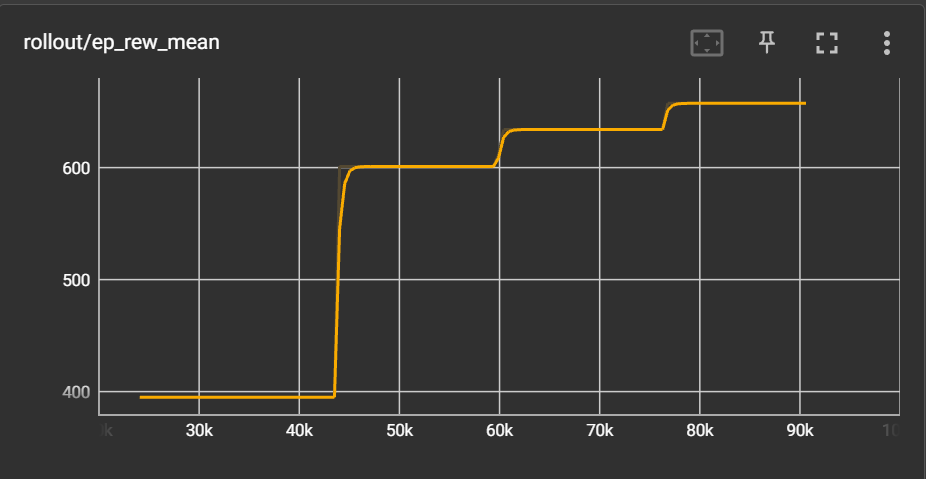
\includegraphics[width=\linewidth]{reward_env1.png}
	\\	
	\vspace{0.1in}
	\textbf{Fig.2:} Mean reward per episode, LR=1e-6, total steps = 100k
	\\
	\label{fig:Fig.3}
\end{figure}


\begin{figure}[H]
	\centering
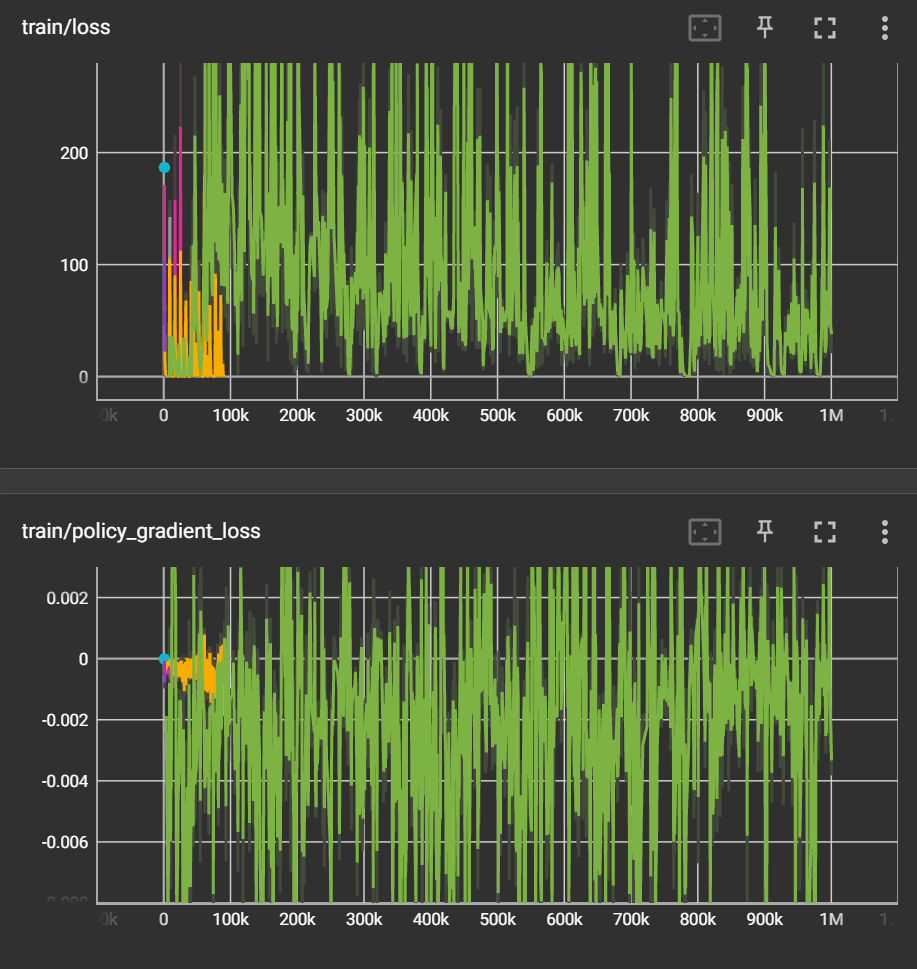
\includegraphics[width=\linewidth]{loss_env1.png}
	\\	
	\vspace{0.1in}
	\textbf{Fig.3:} Policy gradient loss reward per episode, \textbf{Environment 1}
	\\
	\label{fig:Fig.3}
\end{figure}




\subsubsection*{Environment 2}
The second environment responded a lot better from the start. I decided to include more performance plots than the previous one since this was my main environment that I trained most of my models in. The \textbf{learning rate = 0.00003 = 3e-4} was held constant for every model while incrementing the total timesteps for the model. I wanted to include figures that compared every model between each other, rather than performance metrics for each one. I will show the models one by one in the video presentation. For this case however, I wanted to see the general performance of every model at once. First, let me create a legend for Fig.4-6 for the configuration for these models:

\begin{itemize}
\item Model 1, gray: 100k timesteps
\item Model 2, fluorescent blue: 500k timesteps
\item Model 3, light orange: 1 million timesteps
\item Model 4, dark orange: 1.5 million timesteps
\item Model 5, fluorescent green: 2 million timesteps
\item Model 6, matte blue (the one that starts up to in Fig.4): \textbf{Retrained} model 5 with 1 million more timesteps
\item Model 7, red: 4 million timesteps, fresh model

\end{itemize}




\begin{figure}[H]
	\centering
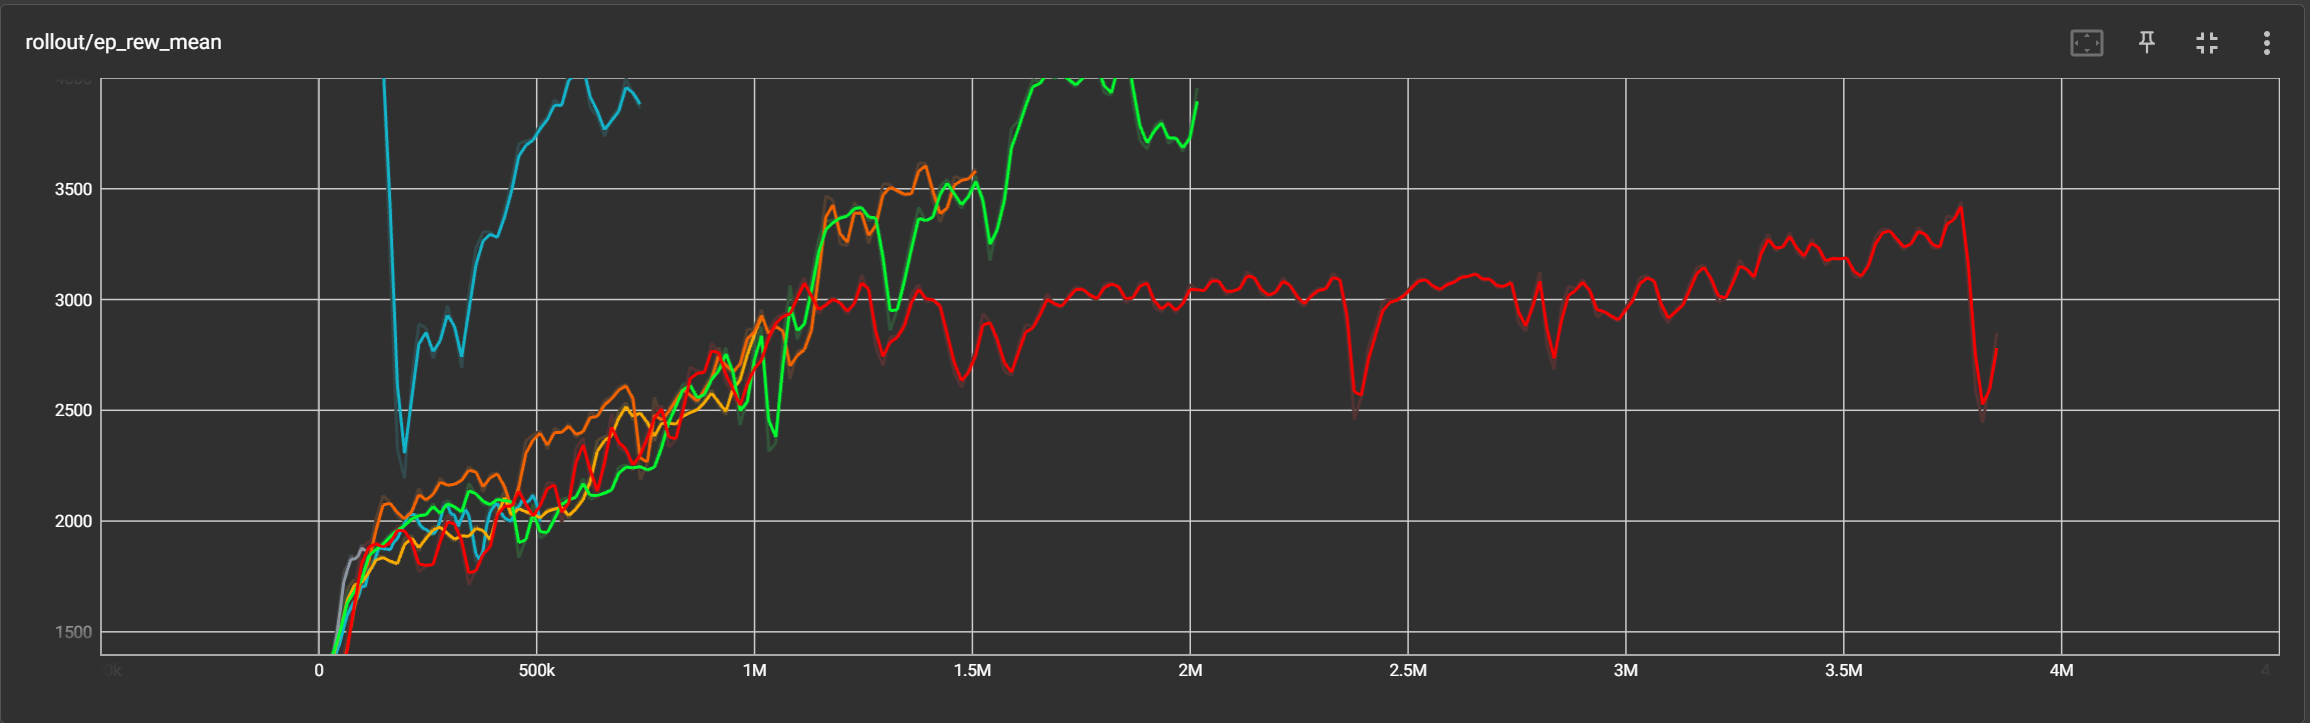
\includegraphics[scale=3,width=\linewidth]{ep_rew_mean_env2.png}
	\\	
	\vspace{0.1in}
	\textbf{Fig.4:} Mean reward per episode, \textbf{Environment 2}
	\\
	\label{fig:Fig.3}
\end{figure}

Fig.4 demonstrates the general performance of the model. We can see a clear trend upwards in with increasing timesteps. The model that achieves the best score is model 5, with 2 million timesteps. Model 6 also reaches that score, however model 6 is a retrained version of model 5. I had hoped that this model would keep on improving model 5 but as we can see in Fig.4., it takes a very wrong turn that results in the reward tanking and takes a while to recover. It also didn't quite seem to finish training since there was a memory issue (included in the Jupyter Notebook). The only explanation I think of is the that the model already took up a lot of space and retraining isn't optimal. Another explanation for could be that this environment performs quite well in the range of 500k-2million timesteps. The mean reward per episode in this interval is similar across every model that I have trained. Perhaps, this environment isn't optimal for handling models that are going to train for $> 2.5 * 10^6$ timesteps. I wanted hoped that this assumption that I had was wrong but the last model that I trained, model 7, couldn't recover from a bad step even after 2 additional timesteps. One last thing I want to point out is the that there is an increase of at least 500 in the score every 500k timesteps. This can be seen in the models 1-5. There are even some bigger jumps that happen, e.g model 5. There is a huge jump in reward from timestep 1 million to timestep 1.5 million. While actually testing the models, I had the best luck with model 4 and model 5. No surprise there since these showed the most consistent performance. They completed the level several times during my test run. I will demonstrate the video in the presentation. 


\begin{figure}[H]
	\centering
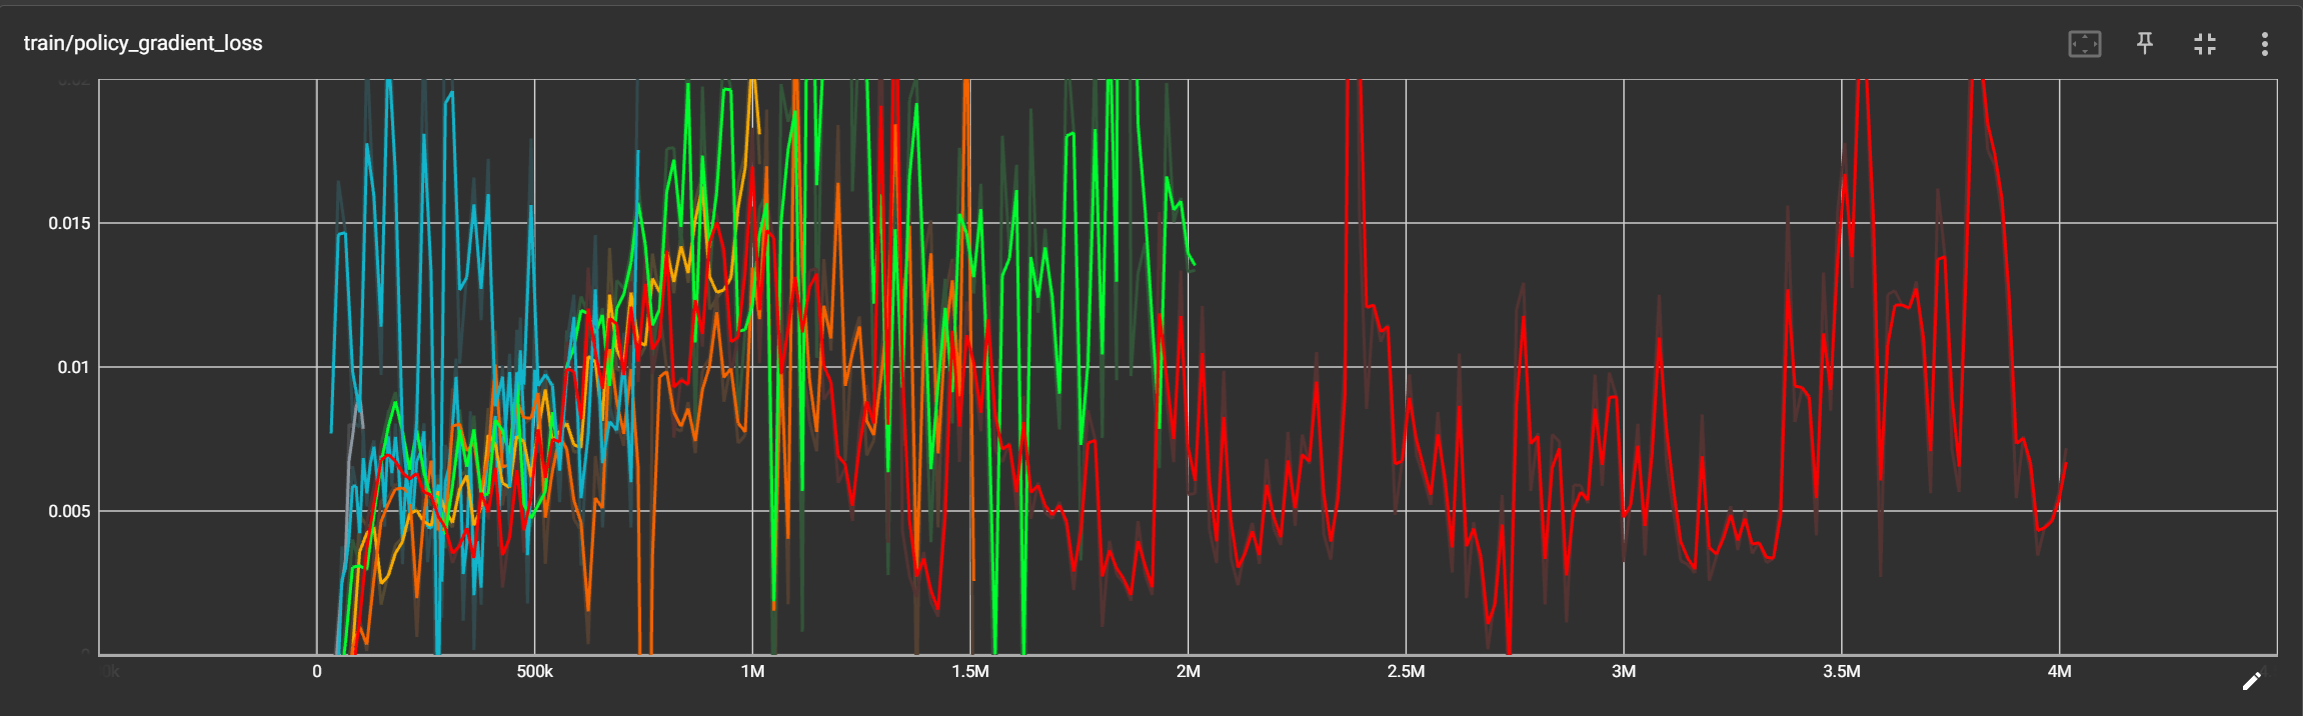
\includegraphics[scale=3,width=\linewidth]{policy_loss_env2.png}
	\\	
	\vspace{0.1in}
	\textbf{Fig.5:} Policy gradient loss per episode, \textbf{Environment 2}
	\\
	\label{fig:Fig.3}
\end{figure}

In Fig.5, we can see the policy gradient loss of each model. As described in the Methods section, the policy gradient loss can be positive or negative, depending on the estimated advantage. We can see this clearly through the ups and downs in each model. In comparison to the first environment, the loss is less fuzzy. The agent keeps taking good, consecutive actions. This doesn't mean that it will always keep making them. However, the general trend of the losses for models 1-5 is upwards, hinting at a better policy. What is interesting is that with model 7 (red), the general trend for the performance in Fig.4 flatlines after 2 million timesteps, just like in Fig.5. Even though there are peaks, the loss doesn't progressively go up. 




\begin{figure}[H]
	\centering
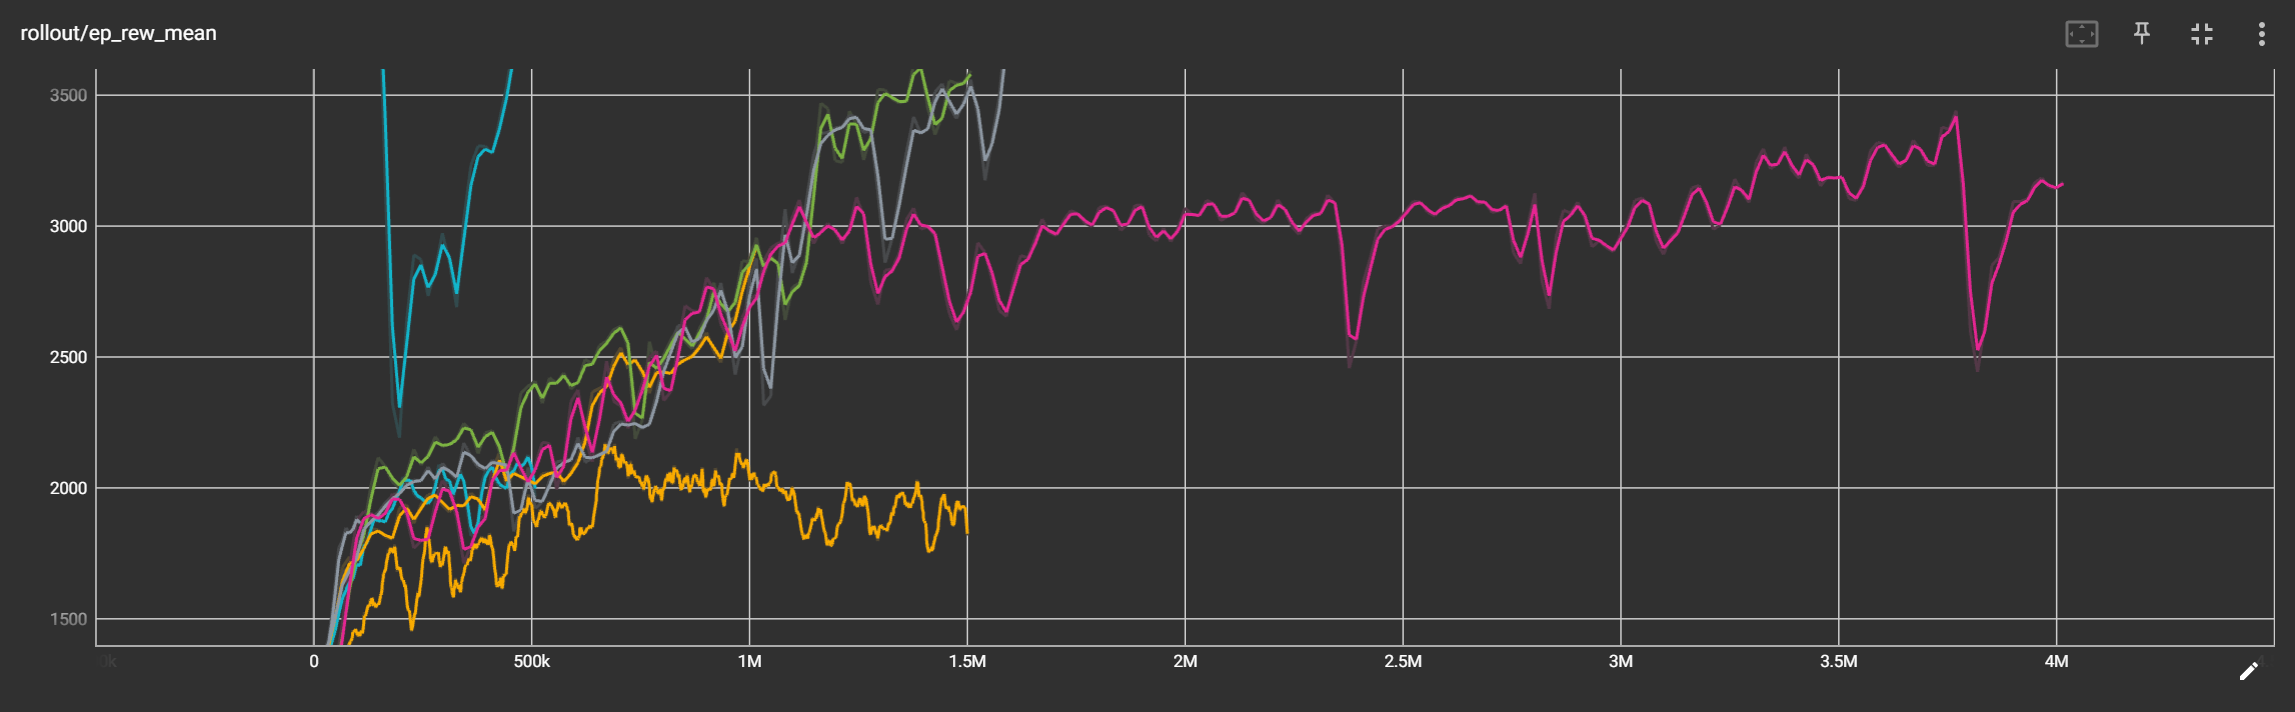
\includegraphics[scale=3,width=\linewidth]{dqn_vs_ppo_env2.png}
	\\	
	\vspace{0.1in}
	\textbf{Fig.7:} DQN (orange) vs. PPOs (rest), \textbf{Environment 2}
	\\
	\label{fig:Fig.3}
\end{figure}

After training model 7 with 4 million timesteps (shown in Fig.4 and Fig.5 as bright red, shown as bright purple in Fig.7), I wanted to check if I PPO was the right solution for this problem. So, I decided to test a DQN as well in this environment. Just like PPO, DQN can be imported from the stable-baselines3 package with ease. The DQN model underperformed every PPO model as we can see in Fig.7. In the first 500-700k timesteps, it is holding up fairly with the PPO models but than cannot push further after 800k. This may be due to the replay buffer that the DQN has to constantly check for. The utilization of the replay buffer/memory holds up a decent chunk in the memory, which in the end could affect the maximum timestep that we can train the model before we hit a plateau, just like the plateau with PPOs at around 2.5 million timesteps. The claim of OpenAi was right in this scenario.




\section*{Conclusion}
In this final project, I have learned how to configure an optimal environment, observe performance metrics and obtain a model that can beat the first level of Super Mario Bros. I have majorly underestimated the significance of fine tuning and environment optimization after completing the CartPole problem since that environment is significantly simpler than this one. I thought that I could train an agent with minimal timesteps and no pre-processing of the environment. Even though this level is simple, the agent still requires a lot of training in order to complete it. I will personally look further into this project in my own free time and extend the training to the whole game so that Mario can beat it in one single run.  




\begin{comment}

\begin{figure}[H]
	\centering
	
	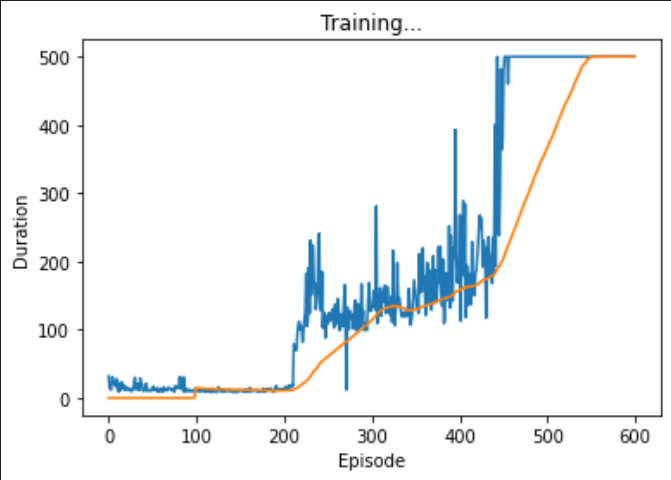
\includegraphics[width=\linewidth,cframe=blue 2.5pt 2.5pt]{agent600.png}
	\\	
	\vspace{0.1in}
	\textbf{Fig.3:} A trained agent with num\_episodes = 600
	\\
	\label{fig:Fig.3}
\end{figure}
\end{comment}













\end{document}